\documentclass[titlepage]{article}
\usepackage[tc]{titlepic}
\usepackage{graphicx}
\usepackage{amsmath}
\usepackage[top=25mm, bottom=25mm, left=27mm, right=27mm]{geometry}
\usepackage{caption}
\usepackage{listings}
\usepackage{lstlangarm}
\usepackage{tabu}
\usepackage[outdir=./]{epstopdf}


\date{}
\author{Erdal Sidal Dogan\\ \#041702023  \and Alp
	Gokcek \\ \#041701014}
\title{\includegraphics[width=0.6\textwidth]{../images/logo_en_color.png}\\ 
\vspace{5em}
EE306 - Microprocessors\\
\vspace{2em}
\textbf{Laboratory Exercise 3 \linebreak Subroutines
}\\
\vspace{1.5em}
March 17, 2020}

\begin{document}
	\maketitle
	\section{Part III - Sigma Sum}
	Sigma Sum explanation
	
	\lstinputlisting[language={[ARM]Assembler}, frame=single, basicstyle=\ttfamily, caption=Assembly Code for sigma sum]{../source_codes/task-iii.s}
	
		\begin{figure}[th]
		\centering
		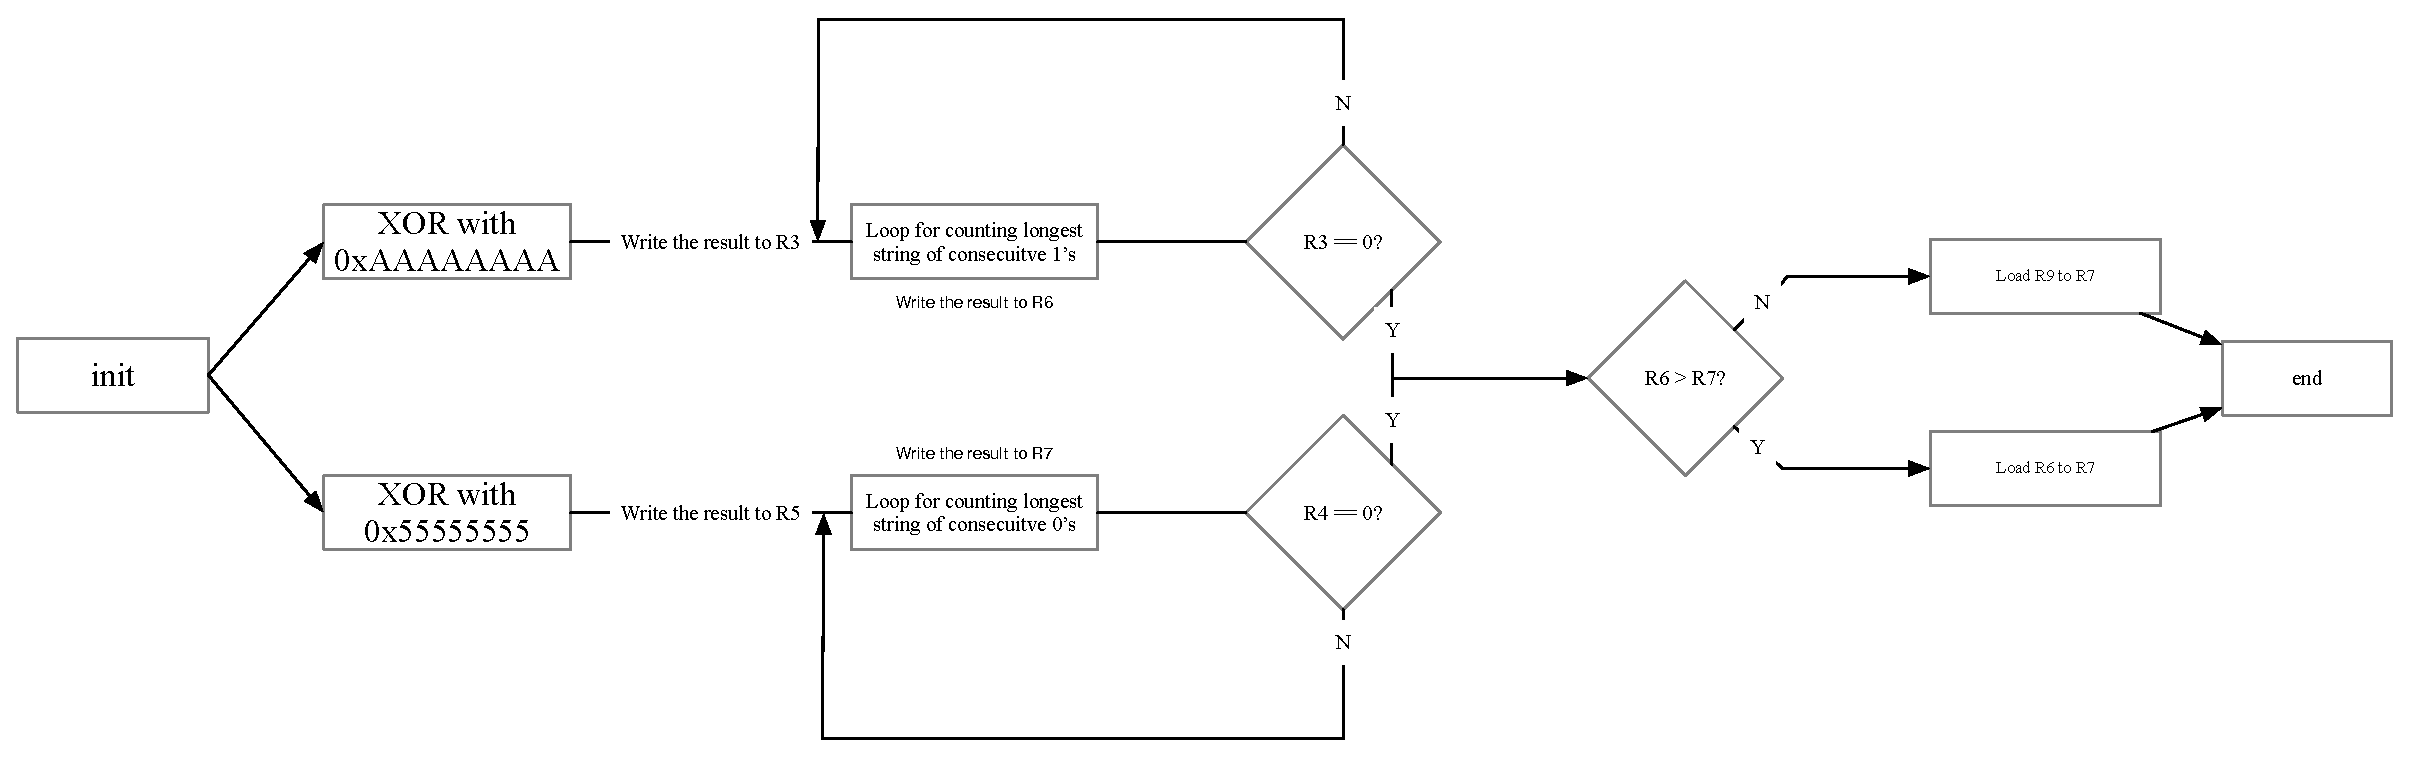
\includegraphics[scale=.4]{../images/task-iii.eps}
		\caption{Longest Sequnce of Alternating 1's and 0's Flowchart}
	\end{figure}

	\section{Part IV - Bubble Sort}
	Bubble sort explanation
	\lstinputlisting[language={[ARM]Assembler}, frame=single, basicstyle=\ttfamily, caption= Assembly code for bubble sort algorithm]{../source_codes/task-iv.s}
	
	\begin{figure}[th]
		\centering
		\includegraphics[scale=.4]{../images/task-iv.eps}
		\caption{Longest Sequnce of Alternating 1's and 0's Flowchart}
	\end{figure}

\end{document}